\objectives{%
  \item define a class of linear hypotheses for given featurized data
  \item compute and efficiently optimize the perceptron and svm losses suffered
        by a hypothesis
}

% -- what hypotheses will we consider?  a recipe for $\hH$
% -- how good is a hypothesis?  fit
% -- which hypothesis is best?  optimization by gradient descent
% -- how good is a hypothesis?  plausibility
% -- two more tasks
% -- improving approximation, optimization, generalization

\sampassage{what hypotheses will we consider?  a recipe for $\hH$}
  Remember: we want our machine to find an input-to-output rule.  We call
  such rules \textbf{hypotheses}.  As engineers, we carve out a menu $\hH$ of
  rules for the machine to choose from.
  %
  We'll consider
  hypotheses of this format:
  \emph{extract features} of the input to make a list of numbers; then
  \emph{linearly combine} those numbers to make another list of numbers;
  finally,
  \emph{read out} a prediction %a distribution over output values
  from the latter list.
  Our digit classifying hypotheses, for instance, look like:\bovinenote{%
    Our list \texttt{threeness} has length one: it's just a fancy way of talking
    about a single number.  We'll later use longer lists to model richer outputs:
    to classify between $>2$ labels,
    to generate a whole image instead of a class label, etc.
  }
  \begin{lstlisting}[language=Python, basicstyle=\footnotesize\ttfamily]
    def predict(x):
      features = [brightness(x), width(x)]              # featurize
      threeness = [ -1.*features[0] +4.*features[1] ]   # linearly combine
      prediction = 3 if threeness[0]>0. else 1          # read out prediction
      return prediction
  \end{lstlisting}
  The various hypotheses differ only in those coefficients (jargon:
  \textbf{weights}, here $-1, +4$) for their linear combinations; it is these
  degrees of freedom that the machine \emph{learns} from data.
  %
  %We can diagram such hypotheses by drawing arrows:
  These arrows summarize the situation:\bovinenote{%
      This triple of arrows is standard in ML.  But the name
      `readout' is not standard jargon.  I don't know standard jargon for this
      arrow.
  }
  \[
    \xX   \xrightarrow[\text{\color{gray}not learned}]{\text{featurize}}
    \Rr^2 \xrightarrow[\text{\textbf{learned!}}]{\text{linearly combine}}
    \Rr^1 \xrightarrow[\text{\color{gray}not learned}]{\text{read out}}
    \yY
    %\text{DistributionsOn}(\yY)
  \]
  %
  Our Unit 1 motto is to \emph{learn linearities flanked by hand-coded
  nonlinearities}.  We design the nonlinearities to capture domain knowledge
  about our data and goals.

  \attnsam{CONFIDENCE}

  For now, we'll assume we've already decided on our featurization and we'll
  use the same readout as in the
  code above:
  \begin{lstlisting}[language=Python, basicstyle=\footnotesize\ttfamily]
      prediction = 3 if threeness[0]>0. else 1
  \end{lstlisting}
  Of course, if we are classifying dogs vs cows that line would read
  \begin{lstlisting}[language=Python, basicstyle=\footnotesize\ttfamily]
      prediction = 'cow' if bovinity[0]>0. else 'dog'
  \end{lstlisting}
  %$$
  %  \texttt{cow if bovinity[0]>0.\ else dog}
  %$$
  In the next three passages we address the key question: \emph{how do we
  determine the weights by which we'll compute \texttt{threeness} or
  \texttt{bovinity} from our features?}.

\sampassage{how good is a hypothesis?  fit}
  We instruct our machine to find within our menu $\hH$ a hypothesis that's as
  ``good'' as possible.  That is, the hypothesis should both fit our training
  data and seem intrinsically plausible.  We want to quantify these notions of
  goodness-of-fit and intrinsic-plausibility.  As with $\hH$, how we quantify
  these notions is an engineering art informed by domain knowledge.  Still,
  there are patterns and principles --- we will study two specific quantitative
  notions, the \textbf{perceptron loss} and \textbf{SVM loss}, to study these
  principles.
  %
  Later, once we understand these notions as quantifying uncertainty (i.e., as
  probabilistic notions), we'll appreciate their logic.  But for now we'll
  bravely venture forth, ad hoc!

  We start with goodness-of-fit.  Hypotheses correspond\bovinenote{%
    A very careful reader might ask: \emph{can't multiple choices of weights
    determine the same hypothesis?}  E.g.\ $(-1, +4)$ and $(-10, +40)$ classify every input
    the same way, since they either both make \texttt{threeness} positive or
    both make \texttt{threeness} negative.
    %
    This is a very good point, dear reader, but at this stage in the course,
    much too pedantic!  Ask again later.
  } to
  weights.  For example, the weight vector $(-1, +4)$ determines the
  hypothesis listed above.

  One way to quantify $h$'s goodness-of-fit to a training example $(x,y)$ is to
  see whether or not $h$ correctly predicts $y$ from $x$.  That is, we could
  quantify goodness-of-fit by \emph{training accuracy}, like we did in the
  previous digits example:
  \begin{lstlisting}[language=Python, basicstyle=\footnotesize\ttfamily]
    def is_correct(x,y,a,b):
      threeness = a*brightness(x) + b*width(x)
      prediction = 3 if threeness>0. else 1
      return 1. if prediction==y else 0.
  \end{lstlisting}
  By historical convention we actually like\bovinenote{%
    ML can be a glass half-empty kind of subject!
  }
  to minimize badness (jargon: \textbf{loss}) rather than
  maximize goodness.  So we'll rewrite the above in terms of mistakes:
  \begin{lstlisting}[language=Python, basicstyle=\footnotesize\ttfamily]
    def leeway_before_mistake(x,y,a,b):
      threeness = a*brightness(x) + b*width(x)
      return +threeness if y==3 else -threeness
    def is_mistake(x,y,a,b):
      return 0. leeway_before_mistake(x,y,a,b)>0. else 1.
  \end{lstlisting}

  We \emph{could} define goodness-of-fit as training accuracy.  But we'll enjoy
  better generalization and easier optimization by allowing ``partial credit''
  for borderline predictions.
  %
  E.g.\ we could use \texttt{leeway\_before\_mistake} as goodness-of-fit:\bovinenote{%
  to define \emph{loss}, we flip signs, hence the `$1-$'
  \exercise{%
    For incentives to point the right way, loss should
    \emph{decrease as \texttt{threeness} increases when \texttt{y==3}} but should
    \emph{increase as \texttt{threeness} increases when \texttt{y==1}}.
    Verify these relations for the several loss functions we define.
  }
  }
  \begin{lstlisting}[language=Python, basicstyle=\footnotesize\ttfamily]
    def linear_loss(x,y,a,b):
      return 1 - leeway_before_mistake(x,y,a,b)
  \end{lstlisting}
  %Notice that if the \texttt{leeway} is very positive, then the badness is
  %very negative (i.e., we are in a very good situation), and vice versa.

  But, continuing the theme of pessimism, we usually feel that a ``very safely
  classified'' point (very positive \texttt{leeway}) shouldn't make up for a
  bunch of ``slightly misclassified'' points (slightly negative
  \texttt{leeway}).\bovinenote{%
    That is,
    %The practical consequence appears during trade-offs:
    we'd rather have \texttt{leeway}s $+.1, +.1, +.1, +.1$
    than $+10, -1, -1, -1$ on four training examples.
    A very positive \texttt{leeway} feels mildly pleasant to us while a
    very negative one feels urgently alarming.
    \exercise compute and compare the training accuracies in these two
    situations.
    %
    %
    As an open-ended followup, suggest reasons why considering
    training \texttt{leeway}s instead of just accuracies might help
    improve testing accuracy.
  }
  But total linear loss
  %incentivizes the opposite choice:
  doesn't capture this asymmetry;
  %
  to address this, let's impose a floor on
  \texttt{linear\_loss} so that it can't get too negative
  (%To cap \texttt{linear\_loss} from below is to
  i.e., so that
    %cap from above how much we care about \texttt{leeway}:
    positive \texttt{leeway} doesn't count arbitrarily much).
    %
    %It's good to get used to this mental flipping between maximizing goodness
    %and minimizing loss.
  We get \textbf{perceptron loss} if we set a floor of $1$; \textbf{SVM loss}
  (also known as \textbf{hinge loss}) if we set a floor of $0$:
  \begin{lstlisting}[language=Python, basicstyle=\footnotesize\ttfamily]
    def perceptron_loss(x,y,a,b):
      return max(1, 1 - leeway_before_mistake(x,y,a,b))
    def svm_loss(x,y,a,b):
      return max(0, 1 - leeway_before_mistake(x,y,a,b))
  \end{lstlisting}

  Proportional weights have the same accuracies but different hinge losses.
  \exercise{Can we say the same of perceptron loss?}
  \begin{figure}[h]
    \centering
    \picturedw{0.23\textwidth}{example-mnist/train-features-hinge-wide-crop.png}%
    \picturew{0.99\textwidth}{bias-trick}%
    \hspace{0.22cm}%
    \picturedw{0.23\textwidth}{example-mnist/train-features-hinge-narrow-crop.png}%
    \hspace{0.22cm}%
    \picturedw{0.46\textwidth}{example-mnist/train-weights-Hinge}
    \caption{%
          \textbf{Hinge loss's optimization landscape reflects confidence, unlike
          training accuracy's.}
          %
          --- \textbf{Left rectangular panes}.  An under-confident and
          over-confident hypothesis.  These have weights
          $(a/3, b/3)$ and $(3a, 3b)$, where
          $(a,b)=(-3.75,16.25)$ minimizes training hinge loss.  The glowing
          colors' width indicates how rapidly \texttt{leeway} changes as we
          move farther from the boundary.
          %
          --- \textbf{Right shaded box}.  The $(a,b)$ plane, centered at the
          origin and shaded by hinge loss, with training optimum {\blu blue}.
          %
          Indecisive $h$s (e.g.\ if
          \texttt{threeness}$\approx 0$) suffer, since $\text{max}(0,1-\ell)\approx
          1$, (not $0$) when $\ell\approx 0$.
          %
          Hinge loss penalizes \emph{overconfident} mistakes severely (e.g.\
          when $y={\blu 1}$ yet \texttt{threeness} is huge):
          $\text{max}(0,1-\ell)$ is unbounded in $\ell$.
          %grows as $\ell$ becomes more negative.
          %
          If we start at the origin $(a,b)=(0,0)$ and shoot (to less
          underconfidence) toward the optimal hypothesis, loss will
          decrease; but once we pass that optimum (to overconfidence),
          loss will (slowly) start increasing again.
    }
  \end{figure}
    %\attnsam{2 PICTURES OF LOSS FUNCTIONS (PLOT vs dec; and PLOT in feature space); illustrate width dependence!!  Weight space?}

\newpage
\sampassage{which hypothesis is best?  optimization by gradient descent}
  Now that we've quantified badness-of-fit-to-data, we want to find a
  hypothesis $h=(a,b)$ that minimizes it.\bovinenote{%
    Soon we'll also include intrinsic implausibility!  We'll see throughout
    this course that it's important to minimize implausibility plus
    badness-of-fit, not just badness-of-fit; otherwise, optimization might
    select a very implausible hypothesis that happens to fit the the training
    data.  Think of the Greek constellations: isn't it miraculous how
    constellations --- the bears, the queen, etc --- so perfectly fit the
    positions of the stars?
  }
  We
  \emph{could} try brute force, as follows:
  \begin{lstlisting}[language=Python, basicstyle=\footnotesize\ttfamily]
    def best_hypothesis():
      # returns a pair (loss value, hypothesis)
      return min(perceptron_loss((training_data, a, b), (a,b))
                 for a in np.arange(-50,+50,.25)
                 for b in np.arange(-50,+50,.25)              )
  \end{lstlisting}
  But this is slow!  Here we're searching a 2D grid at resolution $\approx
  400$, so we call the loss $400^2$ times.  That exponent counts the parameters
  we're finding (here, $2$: $a$ and $b$); if we had $10$ features and $10$
  weights, we'd make $400^{10}$ calls.  Yikes!
  \begin{marginfigure}[-2cm]
    \centering
    \picturedw{0.99\textwidth}{example-mnist/train-weights-HingeReg}
    \caption{%
        \attnsam{REPLACE}
      With $\lambda=0.02$ the objective visibly prefers weights near $0$.
      We develop an algorithm to take steps in this plane
      toward the minimum, `rolling down' the hill so to speak.
    }
  \end{marginfigure}

  Let's instead use more of the information available to direct our search.
  Suppose at some point in our search the best $h$ we've found so far is
  $(a, b)$.  The loss function is a sum (or average) over $N$
  training points $(x_i, y_i)$:\bovinenote{%
    Here, $\text{br}(x)$ and $\text{wi}(x)$ stand for the features of $x$,
    say the brightness and width.
    %
    Also, we'll use take $y$'s values to be $\pm 1$ (rather than cow vs dog
    or {\blu $1$} vs {\rng $3$}), for notational convenience.
  }
  \begin{align*}
      +\max(1,1-{y_{0}}  (a \cdot {\text{br}(x_{0})} + b \cdot{\text{wi}(x_{0})})+\cdots
    \\+\max(1,1-{y_{42}} (a \cdot {\text{br}(x_{42})} + b \cdot{\text{wi}(x_{42})})+\cdots
  \end{align*}

  Let's try to decrease this sum by reducing one row at a time.
  %
  If the row's $\max(1,1-\ell)$ term is $1$, then\bovinenote{%
    except in the negligible case where $\ell=0$ exactly
  }
  any small change in $(a,b)$ won't change that term.
  %
  But if $\max(0,1-\ell)$ term isn't $1$, then we can decrease it by increasing
  $\ell$, i.e., by increasing (say):
  $$
    \underbrace{+1}_{y_{42}}  (a \cdot \underbrace{0.9}_{\text{br}(x_{42})} + b \cdot\underbrace{0.1}_{\text{wi}(x_{42})})
  $$
  We can increase $\ell$ by increasing $a$ or $b$; but increasing $a$ gives us
  more bang for our buck ($0.9>0.1$), so we'd probably nudge $a$ more than $b$,
  say, by adding a multiple of $(+0.9, +0.1)$ to $(a, b)$.  Conversely, if
  ${y_i=-1}$ then we'd add a multiple of $(-0.9, -0.1)$ to $(a, b)$.
  %
  Therefore, to reduce the $i$th row, we want to move $a, b$ like this:
    \emph{Unless the max term is $0$,
      add a multiple of $y_i ({\text{br}(x_{i})}, {\text{wi}(x_{i}))}$ to $(a,b)$.}

  Now, what if improving the $i$th row messes up other rows?  Because of this
  danger we want to take small steps --- i.e., we scale the multiples we
  mention above by some small $\eta$.  That way, even if the rows all pull
  $(a,b)$ in different directions, the dance will buzz close to some average
  $(a,b)$ that minimizes the average row.  So let's initialize
  $h=(a,b)$ arbitrarily and take a bunch of small steps!
  \begin{lstlisting}[language=Python, basicstyle=\footnotesize\ttfamily]
    ETA = 0.01
    h = initialize()
    for t in range(10000):
      xfeatures, y = fetch_datapoint_from(training_examples)
      leeway = y*h.dot(xfeatures)
      h = h + ETA * ( y * xfeatures * (0 if max(1.,1-leeway)==1 else 1) ) # update
  \end{lstlisting}
  \exercise{%
    Convince a friend that, for $\eta=\text{ETA}=1$, this is the
    \textbf{perceptron algorithm} from lecture.
  }
  Choosing smaller $\eta$ means that it takes more steps to get near an optimal
  $h$ but that once we get near we will stay nearby instead of jumping away.
  One can aim for the best of both worlds by letting $\eta$ decay with $t$.
  %Soon we'll formalize and generalize this algorithm using calculus.
  \exercise{%
    We could have used hinge loss instead of perceptron loss.  Mimicking the
    reasoning above, derive a corresponding line of code \texttt{h = h + ...}.
  }


\newpage
\sampassage{how good is a hypothesis?  plausibility}
  Now to define intrinsic plausiblity, also known as a \textbf{regularizer} term.
  There are many intuitions\bovinenote{%
      these come from domain knowledge.  symmetry especially comes to mind.
  }
  but we'll focus for now on capturing this particular intution:
  \emph{a hypothesis that depends very much on very many features is less
  plausible}.
  %
  That is, we find a hypothesis more plausible when its ``total amount of
  dependence'' on the features is small.  We may conveniently quantify this as
  proportional to a sum of squared weights (jargon: \textbf{$L2$}):\bovinenote{%
    We could just as well use $6.86 a^2+b^2$ instead of $a^2+b^2$.
    \exercise{%
      When $(a,b)$ represent weights for brightness-width digits features, how
      how do the hypotheses with small $6.86 a^2+b^2$ visually differ from
      those with small $a^2 + b^2$?
    }
  }
  $
    \text{implausibility of $h=(a,b)$}
    =
    \lambda (a^2 + b^2 + \cdots)
  $.  In code:
  \begin{lstlisting}[language=Python, basicstyle=\footnotesize\ttfamily]
    LAMBDA = 1.
    def implausibility(a,b):
      return LAMBDA * np.sum(np.square([a,b]))
  \end{lstlisting}
  Intuitively, the constant $\lambda$=\texttt{LAMBDA} tells us how much we care
  about plausibility relative to goodness-of-fit-to-data.

  Here's what the formula means.
  Imagine each of three friends has a theory\bovinenote{%
  \textbf{AJ}
    points to wingspan.  A bird with a wings shorter than 1ft can't fly far, so
    it's \emph{sure} to sing instead.  Conversely, birds with longer wings
    never sing.
  \textbf{Pat}
    says to check whether the bird grows red feathers, eats shrimp, lives near
    ice, wakes in the night, and has a bill.  If, of these $5$ qualities, an
    even number are true, then the bird probably sings.  Otherwise, it probably
    doesn't.
  \textbf{Sandy}
uses both wingspan and nocturnality: shorter wings and
    nocturnality both make a bird somewhat more likely to sing.
    }
  about which birds sing.
  %
  Which hypothesis do we prefer?  Well, \textbf{AJ} seems way too confident.
  Maybe they're right that wingspan matters, but it seems implausible that
  wingspan is so decisive.  \textbf{Pat}, meanwhile, doesn't make
  black-and-white claims, but Pat's predictions depend substantively on many
  features: flipping any one quality flips their prediction.  This, too, seems
  implausible.  By contrast, \textbf{Sandy}'s hypothesis doesn't depend too
  strongly on too many features.  To me, a bird non-expert, Sandy's seems most
  plausible.

  Now we can define the overall undesirability of a hypothesis:\bovinenote{%
    We'll use SVM loss but feel free to plug in other losses to get
    different learning behaviors!
  }
  \begin{lstlisting}[language=Python, basicstyle=\footnotesize\ttfamily]
    def objective_function(examples,a,b):
      data_term = np.sum([svm_loss(x,y,a,b) for x,y in examples])
      regularizer = implausibility(a, b)
      return data_term + regularizer
  \end{lstlisting}

  To build intuition about which hypotheses are most desirable according to
  that metric, let's suppose $\lambda$ is a tiny positive number.  Then
  minimizing the objective function is the same as minimizing the data term,
  the total SVM loss: our notion of implausibility only becomes
  important as a tiebreaker.

  \begin{marginfigure}[0cm]
    \centering
    \picturew{0.99\textwidth}{margin}
    \caption{%
      \textbf{Balancing goodness-of-fit against intrinsic plausibility leads
      to hypotheses with large margins.}
      %\textbf{IGNORE the rightmost {\rng orange point} until we say otherwise!}
        A hypothesis's \textbf{margin} is its distance to the closest correctly
        classified training point(s).  Short stems depict these distances for
        two hypotheses (\textbf{black}, {\gre\textbf{gray}}).
        %
        If not for the rightmost {\rng orange point}, we'd prefer \textbf{black} over
        {\gre\textbf{gray}} since it has larger margins.  With large $\lambda$ (i.e., strong
        regularization), we might prefer black over gray even with that
        rightmost {\rng orange point} included, since expanding the margin
        is worth the single misclassification.
      %For convenience we set the origin to the intersection of the two
      %hypotheses.  That way we can still say that every hypothesis's decision
      %boundary goes through
      %the origin.
    }
  \end{marginfigure}

  Now, how does it break ties?  Momentarily ignore the Figure's rightmost {\rng
  orange point} and consider the black hypothesis; its predictions depend only
  on an input's first (vertical) coordinate, so it comes from weights of the
  form $(a,b) = (a,0)$.
  %
  The $(a,0)$ pairs differ in SVM loss.  If
  $a\approx 0$, each point has leeway close to $0$
  and thus SVM loss close to $1$; conversely, if $a$ is huge, each
  point has leeway very positive and thus SVM loss equal to
  the imposed floor: $0$.  So SVM loss is $0$ as long as
  $a$ is so big that each leeway to exceed $1$.

  Imagine sliding a point through the plane.  Its leeway is $0$ at the
  black line and changes by $a$ for every unit we slide vertically.
  %
  So the farther the point is from the black line, the less $a$
  must be before leeway exceeds $1$ --- and the happier is
  the regularizer, which wants $a$ small.
  % TODO BEACH, WATER, SLOPE story
  % TODO Interpreting leeway as a measure of confidence.
  So \emph{minimizing SVM loss with an $L2$ regularizer favors decision
  boundaries far from even the closest correctly classified points!}  The black
  line's margins exceed the gray's, so we favor black.

  For large $\lambda$, then this margin-maximization tendency can be so
  strong that it overrides the data term.  Thus, even when we bring back
  the rightmost {\rng orange point} we ignored, we might prefer the black
  hypothesis to the gray one.

  %That distance is the \textbf{margin}.

%  Now that we've defined our objective function,
%  %(repeated below for easy
%  %reference),
%  we want to find a hypothesis $h=(a,b)$ that minimizes it.  We
%  \emph{could} try brute force, as follows:
%  %  def objective_function(examples,a,b):
%  %    data_term = np.sum([svm_loss(x,y,a,b) for x,y in examples])
%  %    regularizer = implausibility(a, b)
%  %    return data_term + regularizer
%  \begin{lstlisting}[language=Python, basicstyle=\footnotesize\ttfamily]
%    def best_hypothesis():
%      # returns a pair (objective-function value, hypothesis)
%      return min((objective_function(training_data, a, b), (a,b))
%                 for a in np.arange(-50,+50,.25)
%                 for b in np.arange(-50,+50,.25)                 )
%  \end{lstlisting}
%  But this is slow!  Here we're searching a 2D grid at resolution $\approx 400$, so
%  we call the objective function $400^2$ times.  That exponent
%  counts the number of parameters we're finding --- here, we seek
%  $2$ weights $a$ and $b$, but if we had $10$ features and $10$ weights,
%  we'd make $400^{10}$ calls.  Yikes!
%  \begin{marginfigure}[-2cm]
%    \centering
%    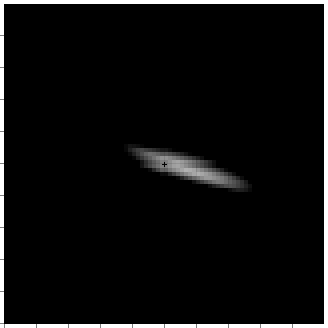
\includegraphics[width=0.99\textwidth]{example-mnist/train-weights-HingeReg}
%    \caption{%
%      With $\lambda=0.02$ the objective visibly prefers weights near $0$.
%      We develop an algorithm to take steps in this plane
%      toward the minimum, `rolling down' the hill so to speak.
%    }
%  \end{marginfigure}
%
%  Let's instead use more of the information available to direct our search.
%  Suppose at some point in our search the best $h$ we've found so far is
%  $(a, b)$.  The objective function is an implausibility plus, for each of $N$
%  training points $(x_i, y_i)$, a badness-of-fit:\bovinenote{%
%    Here, $\text{br}(x)$ and $\text{wi}(x)$ stand for the features of $x$,
%    say the brightness and width.
%    %
%    Also, we'll use take $y$'s values to be $\pm 1$ (rather than cow vs dog
%    or {\blu $1$} vs {\rng $3$}), for notational convenience.
%  }
%  \begin{align*}
%    %  +(\lambda/N)(a^2+b^2)&+\max(0,1-y_0  (a \cdot {\text{br}(x_0)} + b \cdot{\text{wi}(x_0)}) + \cdots
%      +(\lambda/N)(a^2+b^2)&+\max(0,1-{y_{0}}  (a \cdot {\text{br}(x_{0})} + b \cdot{\text{wi}(x_{0})})+\cdots
%    %\\+\cdots&
%    %\\+(\lambda/N)(a^2+b^2)&+\max(0,1-{y_{41}}  (a \cdot {\text{br}(x_{41})} + b \cdot{\text{wi}(x_{41})})
%    \\+(\lambda/N)(a^2+b^2)&+\max(0,1-{y_{42}}  (a \cdot {\text{br}(x_{42})} + b \cdot{\text{wi}(x_{42})})+\cdots
%    %\\+\cdots&
%  \end{align*}
%
%  Let's try to decrease this sum by reducing one row at a time.
%  Well, we can reduce a row's $\lambda/N$ term by moving $a,b$ closer to $0$.
%  %
%  If the row's $\max(0,1-\ell)$ term is $0$, then\bovinenote{except in the
%  negligible case where $\ell=0$ exactly} any small change in $(a,b)$ won't
%  change that term.
%  %
%  But $\max(0,1-\ell)$ term isn't $0$, then we can decrease it by increasing
%  $\ell$, i.e., by increasing (say):
%  $$
%    \underbrace{+1}_{y_{42}}  (a \cdot \underbrace{0.9}_{\text{br}(x_{42})} + b \cdot\underbrace{0.1}_{\text{wi}(x_{42})})
%  $$
%  We can increase $\ell$ by increasing $a$ or $b$; but increasing $a$ gives us
%  more bang for our buck ($0.9>0.1$), so we'd probably nudge $a$ more than $b$,
%  say, by adding a multiple of $(+0.9, +0.1)$ to $(a, b)$.  Conversely, if
%  ${y_i=-1}$ then we'd add a multiple of $(-0.9, -0.1)$ to $(a, b)$.
%  %
%  Therefore, to reduce the $i$th row, we want to move $a, b$ like this:
%    Add a multiple of $(-a,-b)$ to $(a,b)$; and, unless the max term is $0$,
%      add a multiple of $y_i ({\text{br}(x_{i})}, {\text{wi}(x_{i}))}$ to $(a,b)$.
%  %\begin{description}
%  %\item[to reduce the $\max$ term]: {if the max term is $0$, don't do anything.
%  %   Otherwise, add a multiple of $y_i ({\text{br}(x_{i})}, {\text{wi}(x_{i}))}$ to $(a,b)$}
%  %\item[to reduce the $\lambda/N$ term]: {}
%  %\end{description}
%
%  Now, what if improving the $i$th row messes up other rows?  Because of this
%  danger we want to take small steps --- i.e., we scale the multiples we mention above
%  by some small $\eta$.  That way, even if the rows all pull $(a,b)$ in
%  different directions, the dance will buzz close to some average $(a, b)$
%  that maximizes the average row's happiness.  So let's initialize $(a,b)$
%  arbitrarily and take a bunch of small steps!\bovinenote{%
%      \noparexercise{We could have used perceptron loss instead of hinge loss.  Mimicking
%  the reasoning above, derive the familiar perceptron update.  For simplicity
%  let $\lambda=0, \eta=1$.
%  }
%  }
%  \begin{lstlisting}[language=Python, basicstyle=\footnotesize\ttfamily]
%    ETA = 0.01
%    ab = initialize()
%    for t in range(10000):
%      xfeatures, y = fetch_datapoint_from(training_examples)
%      ab = ab + ETA * ( - L * ab
%                        + y * xfeats * (0 if max(0., y*ab.dot(xfeatures))==0 else 1) )
%  \end{lstlisting}
%  This is the \textbf{pegasos algorithm} we'll see in the project.
%  Soon we'll formalize and generalize this algorithm using calculus.




% solving other classification tasks by the same method
\sampassage{worked example: bovinity of reddit posts}
  Digits are nice.  Let's solve a couple other tasks by the same method.  This
  illustrates which aspects are design decisions and which aren't.  We'll start
  with a text-classification task.

  %\textbf{reddit posts about cows vs dogs}
  We gather the text of 2000 reddit posts, half from \texttt{r/Cows} and half
  from \texttt{r/Dogs}.  \emph{Can we predict from text alone which of the two
  subreddits a post came from?}

  Intuitively, words like
  \texttt{cow},
  \texttt{dog},
  \texttt{hoof},
  \texttt{paw},
  \texttt{moo},
  \texttt{bark}
  are tell-tale signs.  So for our featurization, let's have a feature for
  each $3$-letter and each $4$-letter word.  The feature for the word
  \texttt{hoof} simply maps a text input $x$ in $\xX$ to a real number that's
  $1$ if the word appears in the post and $0$ otherwise.  Likewise with the
  other features.

\sampassage{worked example: seeing around walls}
  %\textbf{seeing around walls}
  Let's collect 200 photos of a certain MIT hallway corner.  In half, there's
  some large obstacle (e.g.\ a person) right around the corner.  In the other
  half, there's no obstacle.  \emph{Can we distinguish these cases from pixels
  alone?}

  Intuitively, if this prediction is possible it'd be based on subtle shading
  arising from multiple reflection of light.  So we'll probably want to
  prioritize features to do with brightness.  

% TODO : integrate approximation, optimization, generalization
% into these two examples
%\sampassage{improving approximation, optimization, generalization}

